\documentclass[12pt, letterpaper]{../assignment}
\usepackage{graphicx}
\usepackage{courier}
\usepackage{minted}
\usepackage{amsmath}
\usepackage{commath}
\usepackage{amssymb}
\usepackage{amsfonts} 
\usepackage{cancel}
\usepackage{enumitem}
\usepackage{array}

\usepackage{tikz}
\usetikzlibrary{shapes,arrows,positioning}

\usemintedstyle{monokai}
\oddsidemargin = 0pt
\exercisesheet{Module 9}{Practice Assignment}
\student{Austin Barrilleaux}
\courselabel{EN 525.609}
\semester{Fall 2023}
\usepackage[backend=bibtex,style=numeric,sorting=none]{biblatex}
\bibliography{reference}
\usepackage{color}
\definecolor{light-gray}{rgb}{0.2,0.2,0.2}
\setminted{bgcolor=light-gray}
\setlength{\parindent}{0pt}

\makeatletter
\patchcmd{\minted@colorbg}{\noindent}{\medskip\noindent}{}{}
\apptocmd{\endminted@colorbg}{\par\medskip}{}{}
\makeatother

\begin{document}
\subsection*{Problem 1}
\subsubsection*{Solve the following practice problems in the 9th edition textbook.\\
\begin{itemize}
    \item Chapter 8:
    \begin{itemize}
        \item 8-1
        \item 8-5
    \end{itemize}
\end{itemize}}

\subsubsection*{(8-1) The forward-path transfer function of a unity-feedback control system is:
\boldmath{$$ G(s) = \frac{K}{s (s+6.54)} $$}
Analytically, find the resonance peak \boldmath{$Mr$}, resonant frequency \boldmath{$\omega_r$}, and bandwidth \boldmath{$BW$} of the closed- loop system for the following values of K:}
\subsubsection*{ (a) \boldmath{$K = 5$} }

The prototype second-order forward-path transfer function is:

$$ G(s) = \frac{\omega_n^2}{s ( s + 2 \zeta \omega_n) } $$

From this, we can see that:

$$ \omega_n = \sqrt{K} = \sqrt{5} $$

$$ \zeta = \frac{6.54}{2 \omega_n} = \frac{6.54}{2 \sqrt{5}} = 1.4624 $$

Because $\zeta > 0.707$:

\begin{answer}
    $$ M_r = 1 $$
    $$ \omega_r = 0 $$
\end{answer}

From the text, for the prototype second-order system:

\begin{equation*}
    \begin{aligned}
        BW &= \omega_n \left[ (1 - 2 \zeta^2) + \sqrt{ 4 \zeta^4 - 4 \zeta^2 + 2 } \right]^{\frac{1}{2}}\\
           &= \sqrt{5} \left[ (1 - 2 \cdot 1.4624^2) + \sqrt{ 4 \cdot 1.4624^4 - 4 \cdot 1.4624^2 + 2 } \right]^{\frac{1}{2}}
    \end{aligned}
\end{equation*}

\begin{answer}
    $$ BW = 0.8636 $$
\end{answer}

We can verify these using build in MATLAB functions,\texttt{getPeakGain()} and\\ \texttt{bandwidth()}:

\begin{equation*}
    \begin{aligned}
        [M_r,\omega_r] &= \texttt{getPeakGain([5],[1,6.45,5])}\\
        M_r &= 1.0000\\
        \omega_r &= 0.0000
    \end{aligned}
\end{equation*}

\begin{equation*}
    \begin{aligned}
        BW &= \texttt{bandwidth([5],[1,6.45,5])}\\
        BW &= 0.8616
    \end{aligned}
\end{equation*}

Note that the methodologies for these functions are different from the equations in the book,
so they differ slightly but are close enough to show that our answers are correct approximations.

\subsubsection*{ (b) \boldmath{$K = 21.39$} }

From this, we can see that:

$$ \omega_n = \sqrt{K} = \sqrt{21.39} $$

$$ \zeta = \frac{6.54}{2 \omega_n} = \frac{6.54}{2 \sqrt{5}} = 0.707 $$

Because $\zeta$ is equal to $0.707$, from the textbook:

$$ M_r = \frac{1}{2 \zeta \sqrt{1- \zeta^2}} = 0.648$$

\begin{answer}
    $$ M_r = 1.0000 $$
\end{answer}

$$ \omega_r = \omega_n \sqrt{1- \zeta^2} = 0.648$$

\begin{answer}
    $$ \omega_r = 0.0648 $$
\end{answer}

From the text, for the prototype second-order system:

\begin{equation*}
    \begin{aligned}
        BW &= \omega_n \left[ (1 - 2 \zeta^2) + \sqrt{ 4 \zeta^4 - 4 \zeta^2 + 2 } \right]^{\frac{1}{2}}\\
           &= \sqrt{21.39} \left[ (1 - 2 \cdot 0.707^2) + \sqrt{ 4 \cdot 0.707^4 - 4 \cdot 0.707^2 + 2 } \right]^{\frac{1}{2}}
    \end{aligned}
\end{equation*}

\begin{answer}
    $$ BW = 4.6254 $$
\end{answer}

We can verify these using build in MATLAB functions,\texttt{getPeakGain()} and\\ \texttt{bandwidth()}:

\begin{equation*}
    \begin{aligned}
        [M_r,\omega_r] &= \texttt{getPeakGain([21.39],[1,6.45,21.39])}\\
        M_r &= 1.0000\\
        \omega_r &= 0.0000
    \end{aligned}
\end{equation*}

\begin{equation*}
    \begin{aligned}
        BW &= \texttt{bandwidth([21.39],[1,6.45,21.39])}\\
        BW &= 4.6199
    \end{aligned}
\end{equation*}

Noticing that the $\omega_r$ values are different, I noticed that:

$$ \zeta = \frac{6.54}{2 \omega_n} = \frac{6.54}{2 \sqrt{5}} = 0.707037 $$

Which means that if you don't round $\zeta$, $\zeta$ is greater than $0.707$,
so the function is making $\omega_r$ equal to zero.
Otherwise, our results match MATLAB nicely.
\\\\
Note the comment on the MATLAB functions in the answer for par (a).

\subsubsection*{ (c) \boldmath{$K = 100$} }


From this, we can see that:

$$ \omega_n = \sqrt{K} = \sqrt{100} = 10 $$

$$ \zeta = \frac{6.54}{2 \omega_n} = \frac{6.54}{2 \sqrt{100}} = 0.327 $$

Because $\zeta$ is less than $0.707$, from the textbook:

$$ M_r = \frac{1}{2 \zeta \sqrt{1- \zeta^2}} = 1.618$$

\begin{answer}
    $$ M_r = 1.6180 $$
\end{answer}

$$ \omega_r = \omega_n \sqrt{1- \zeta^2} = 8.866$$

\begin{answer}
    $$ \omega_r = 8.8665 $$
\end{answer}

From the text, for the prototype second-order system:

\begin{equation*}
    \begin{aligned}
        BW &= \omega_n \left[ (1 - 2 \zeta^2) + \sqrt{ 4 \zeta^4 - 4 \zeta^2 + 2 } \right]^{\frac{1}{2}}\\
           &= \sqrt{100} \left[ (1 - 2 \cdot 0.327^2) + \sqrt{ 4 \cdot 0.327^4 - 4 \cdot 0.327^2 + 2 } \right]^{\frac{1}{2}}
    \end{aligned}
\end{equation*}

\begin{answer}
    $$ BW = 14.3463 $$
\end{answer}

We can verify these using build in MATLAB functions,\texttt{getPeakGain()} and\\ \texttt{bandwidth()}:

\begin{equation*}
    \begin{aligned}
        [M_r,\omega_r] &= \texttt{getPeakGain([21.39],[1,6.45,21.39])}\\
        M_r &= 1.6180\\
        \omega_r &= 8.8789
    \end{aligned}
\end{equation*}

\begin{equation*}
    \begin{aligned}
        BW &= \texttt{bandwidth([21.39],[1,6.45,21.39])}\\
        BW &= 14.3398
    \end{aligned}
\end{equation*}

Noticing that the $\omega_r$ values are different, I noticed that:

$$ \zeta = \frac{6.54}{2 \omega_n} = \frac{6.54}{2 \sqrt{5}} = 0.707037 $$

Our results match MATLAB nicely.
\\\\
Note the comment on the MATLAB functions in the answer for par (a).

\subsubsection*{(8-5) The specifications on a second-order unity-feedback control system with the closed-loop transfer function:
\boldmath{$$ M(s) = \frac{Y(s)}{R(s)} = \frac{\omega_n^2}{s^2 + 2 \zeta \omega_n s + \omega_n^2} $$}
are that the maximum overshoot must not exceed 10\% and the rise time must be less than 0.1 sec. Find the corresponding limiting values of $M_r$ and $BW$ analytically.}

From the textbook:

$$ \text{maximum overshoot} = e^\frac{-\pi\zeta}{\sqrt{1- \zeta^2}} $$

Which can be rearranged as:

$$ \zeta = \sqrt{\frac{\ln(\text{maximum overshoot})^2}{(\pi^2 + \ln(\text{maximum overshoot})^2)}} $$

$$ \zeta = \sqrt{\frac{\ln(\text{0.1})^2}{(\pi^2 + \ln(\text{0.1})^2)}} = 0.5912 $$

Because $\zeta$ is less than $0.707$, from the textbook:

$$ M_r = \frac{1}{2 \zeta \sqrt{1- \zeta^2}} = 1.0487$$

\begin{answer}
    $$ M_r = 1.0487 $$
\end{answer}

Using rise time to solve for $\omega_n$, from the textbook:

$$ t_r = \frac{1 - 0.4167 \zeta + 2.917 \zeta^2}{\omega_n}$$

Rearranging for $\omega_n$:

\begin{equation*}
    \begin{aligned}
        \omega_n &= \frac{1 - 0.4167 \zeta + 2.917 \zeta^2}{t_r}\\
                 &= \frac{1 - 0.4167 (0.5912) + 2.917 (0.5912)^2}{t_r}\\
                 &= 17.7305
    \end{aligned}
\end{equation*}


The bandwidth is calculated as:

\begin{equation*}
    \begin{aligned}
        BW &= \omega_n \left[ (1 - 2 \zeta^2) + \sqrt{ 4 \zeta^4 - 4 \zeta^2 + 2 } \right]^{\frac{1}{2}}\\
           &= 17.7305 \left[ (1 - 2 \cdot 0.5912^2) + \sqrt{ 4 \cdot 0.5912^4 - 4 \cdot 0.5912^2 + 2 } \right]^{\frac{1}{2}}
    \end{aligned}
\end{equation*}

\begin{answer}
    $$ BW = 26.5660$$
\end{answer}

\subsection*{Problem 2}
\subsubsection*{Construct the Bode plot for the following open-loop transfer function
of a unity-feedback system:}

$$ \mathbf{G(j\omega) = \frac{10(1+j\omega)}{(j\omega)^2 \left( 1 + \frac{j\omega}{4} + \left(\frac{j\omega}{4}\right)^2\right) } }$$


\subsubsection*{(a) First by hand using the rules developed in this module}

The makeup of the bode plot will consist of four parts.
\\\\
The transfer function has a constant $K=10$. This component will have a constant magnitude of:

$$ K_\text{dB} = 20 \log_{10} |K| = 20 \log_{10} |10| = 20 $$

Since $K > 0$ the angle for this component is $0$.
\\\\
There is a pole at the origin who's component will have a magnitude which is a constant slope of
$-20 r = -40 $ db/decade. Its phase is $-r90 = -180$.
\\\\
There is a real axis zero who's magnitude is equal to zero until the frequency equals break frequency of 1,
then ramps up to a slope of $20$ db/decade. Its angle starts at an asymptote of zero,
then at a break frequency equal to 0.1 approaches an inflection point of $45^\circ$ at frequency equal to $1$, after a break frequency equal to 10 it
then approaches an asymptote of $90^\circ$.
\\\\
There is a quadratic pole who's magnitude is equal to zero until the frequency equals 4,
then ramps down to a slope of $-40$ db/decade.
Its angle starts at an asymptote of zero,
then at a break frequency equal to 1 approaches an inflection point of $-90^\circ$, after which it
then approaches an asymptote of $-180^\circ$.
\\\\
The magnitude of the bode plot is reflected in the following plot:

\begin{figure}[H]
    \centering
    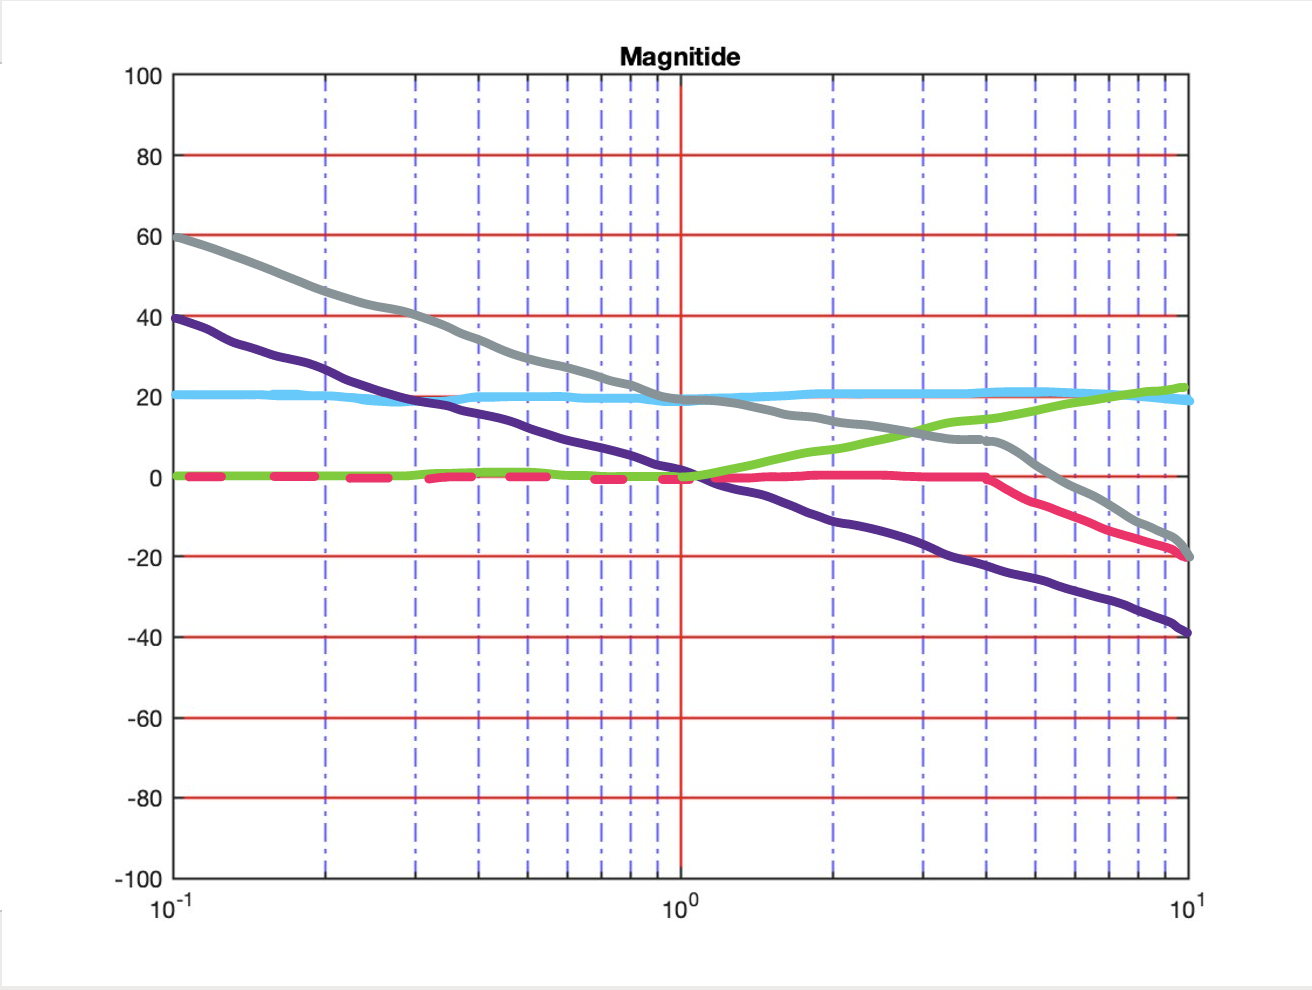
\includegraphics[width=0.7\linewidth]{./figures/Magnitude.png}
    \caption{Magnitude}
    \label{fig:step}
 \end{figure}

 The phase of the bode plot is reflected in the following plot:

\begin{figure}[H]
    \centering
    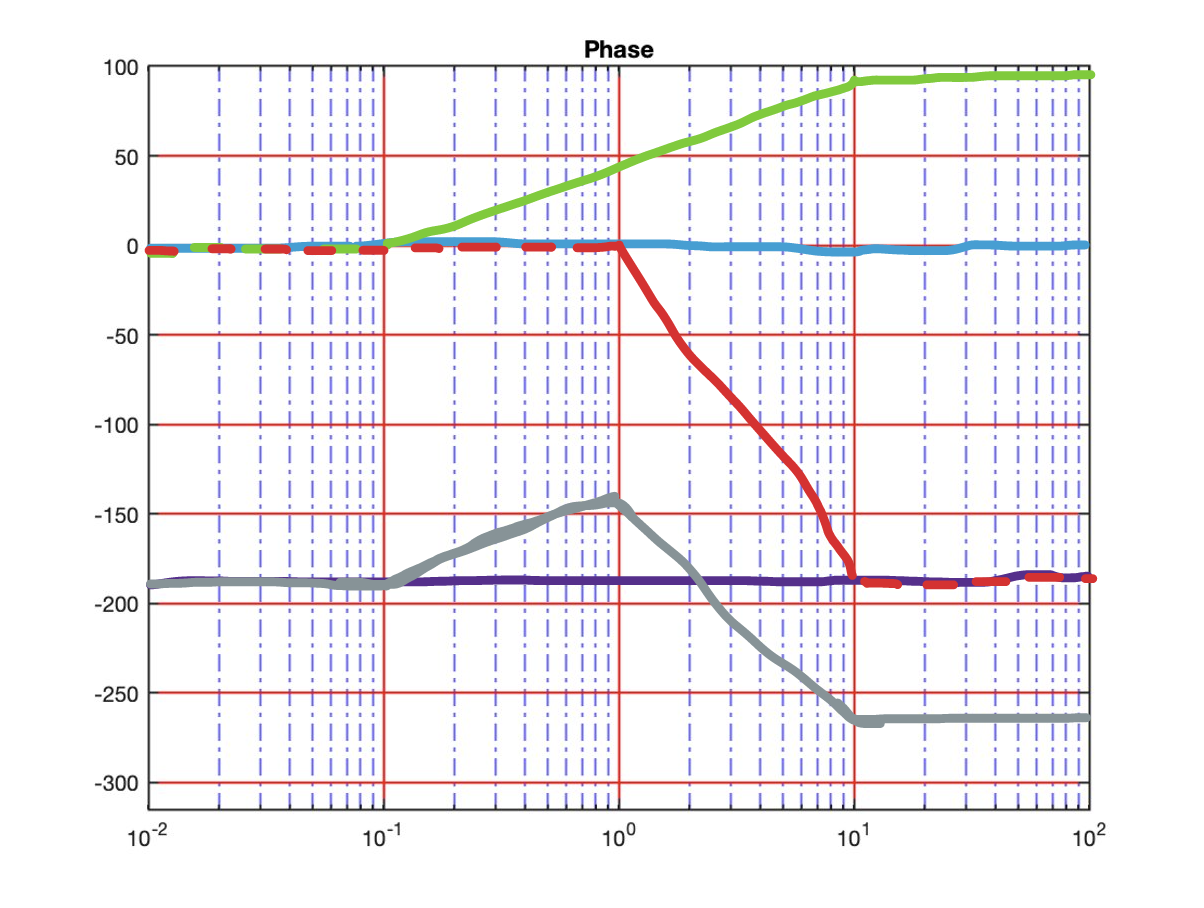
\includegraphics[width=0.6\linewidth]{./figures/Phase.png}
    \caption{Magnitude}
    \label{fig:step}
 \end{figure}

In both plots, the grey line reflects the composite of the discussed constituent parts.

\subsubsection*{(b) Using the “bode” command in MATLAB}

Using the “bode” command in MATLAB produced the following plot:

\begin{figure}[H]
    \centering
    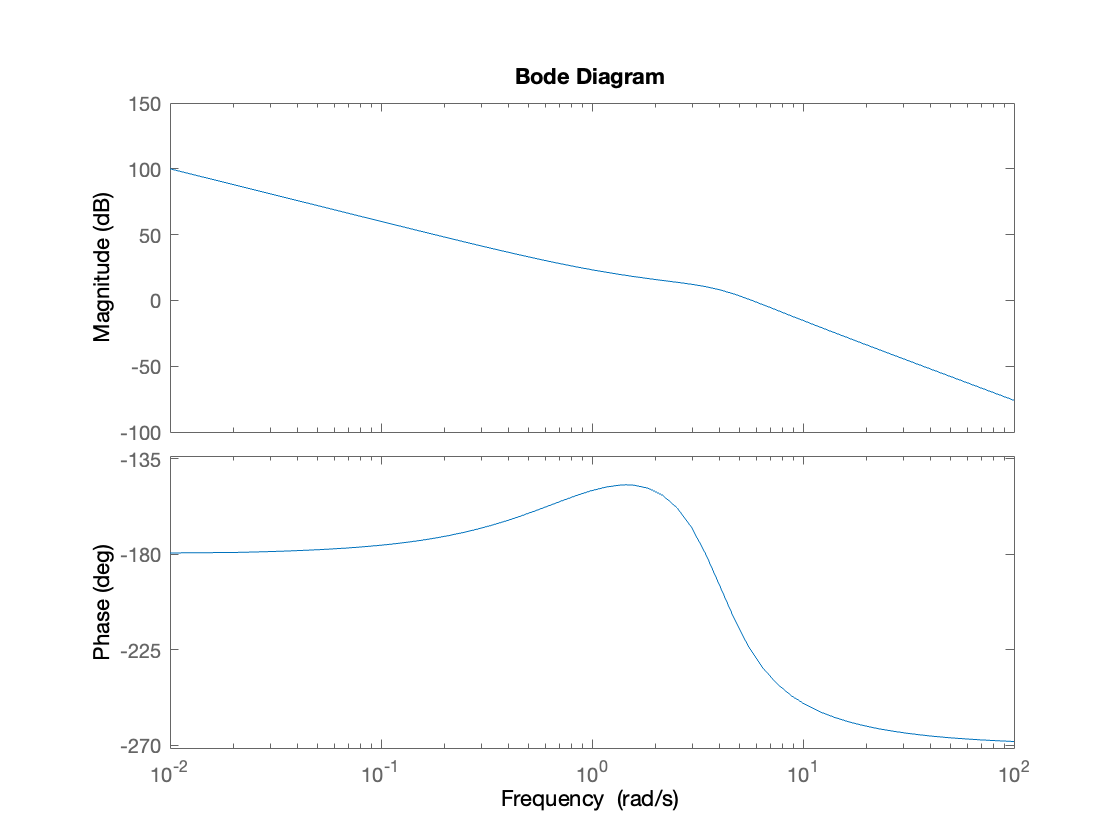
\includegraphics[width=0.6\linewidth]{./figures/matlab_bode.png}
    \caption{Bode Plot}
    \label{fig:step}
 \end{figure}

 Both sets of plots match each other.
  
% \color{white}
% \hspace*{6em}\inputminted[frame=leftline,fontsize=\footnotesize]{matlab}
% {./matlab/Problem_5_18.m}
% \color{black}

% \begin{figure}[H]
%     \centering
%     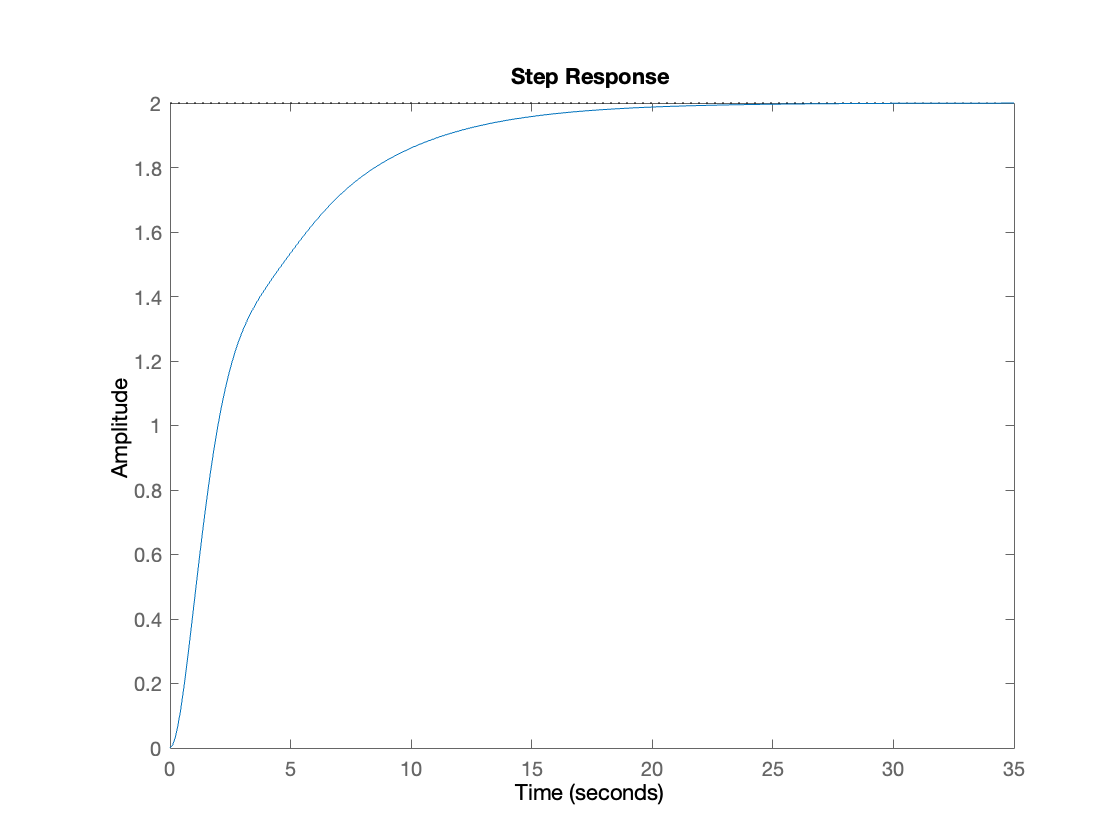
\includegraphics[width=0.7\linewidth]{./figures/step_response.png}
%     \caption{Step Response}
%     \label{fig:step}
%  \end{figure}



\end{document}

